% !TeX spellcheck = it_IT
\newpage
\section{Analisi dei requisiti}
\begin{definition}
	Processo di studio e analisi delle esigenze del committente e dell'utente per giungere alla definizione del dominio del problema e dei requisiti del sistema.
\end{definition}
L'analisi serve a capire \textbf{cosa} fare e non come farlo, identificando i confini del sistema SW, il modo in cui interagisce con l'ambiente e la qualità con cui lo fa.\\
È un processo \textbf{fondamentale} in quanto permette di individuare e risolvere difetti in maniera meno costosa rispetto alle altre fasi di sviluppo software.\\
Il prodotto dell'analisi dovrà essere un documento e/o modello che descrive il \textbf{dominio} del sistema, i suoi \textbf{requisiti} ed opzionalmente il \textit{manuale utente} e i \textit{casi di test}.
\subsection{Studio di fattibilità}
È la fase preliminare per stabilire l'opportunità di realizzare o meno un sistema software. Si basa su:
\begin{itemize}
	\item \textbf{Descrizione} del sistema e delle necessità degli utenti
	\item Analisi di \textbf{mercato}:
	\begin{itemize}
		\item Mercato \textit{attuale} e \textit{futuro}
		\item \textit{Costo} di produzione
		\item \textit{Redditività} attesa
	\end{itemize}
	\item Analisi tecnica di \textbf{realizzabilità}:
	\begin{itemize}
		\item Strumenti necessari
		\item Soluzioni algoritmiche e architetturali
		\item Hardware
		\item Processo
	\end{itemize}
\end{itemize}

\subsection{Dominio}
Per la costruzione del dominio sono necessari:
\begin{itemize}
	\item Un \textbf{glossario}: collezione di termini rilevanti al caso specifico. Costruito strada facendo dagli analisti e può essere riutilizzato.
	\item Modello \textbf{statico} e \textbf{dinamico}
\end{itemize}
Ci si deve concentrare su: \textbf{entità}, \textbf{relazioni}, \textbf{processi} e \textbf{comportamenti}.

\begin{example}[House of cars]
	House of Cars è un parcheggio verticale multipiano, formato da 10 colonne e 24 piani per colonna, 12 sotto al livello strada e 12 sopra.
	
	\paragraph{Glossario}
	\begin{itemize}
		\item \textit{Colonna}: colonna di posti auto dotata di un sollevatore centrale che raggiunge tutti i piani del parcheggio; ha un proprio locale di ricezione auto; comprende un carrello
		\item \textit{Carrello}: carrello per movimentare le vetture; è dotato di “forchette” in corrispondenza delle ruote
		\item \textit{Cella}: formata da due box affiancati: può quindi contenere due auto
		\item \textit{Gruppo di spostamento elettromeccanico}: controlla il carrello che trasla la vettura nelle celle posizionate davanti e dietro al sollevatore
		\item  $\ldots$
	\end{itemize}
	
	\begin{center}
		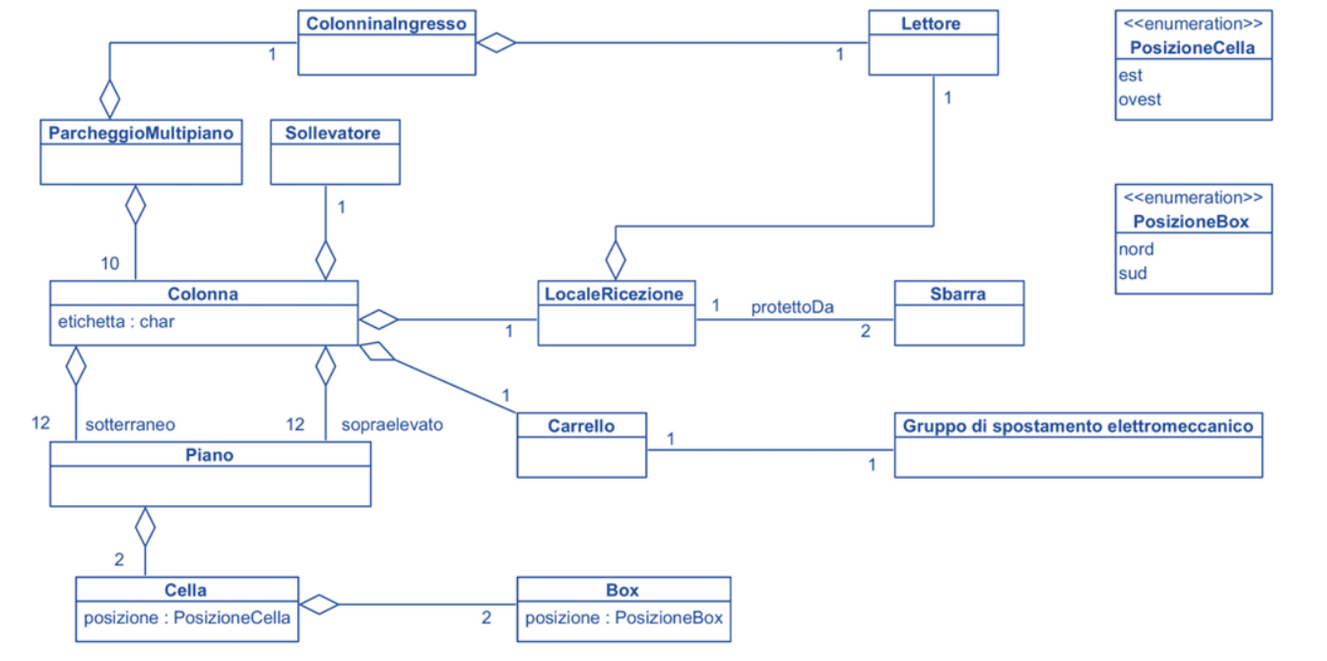
\includegraphics[scale=0.3]{smodelhousecars.png}
		\captionof{figure}{Modello statico}
	\end{center}
	\begin{center}
		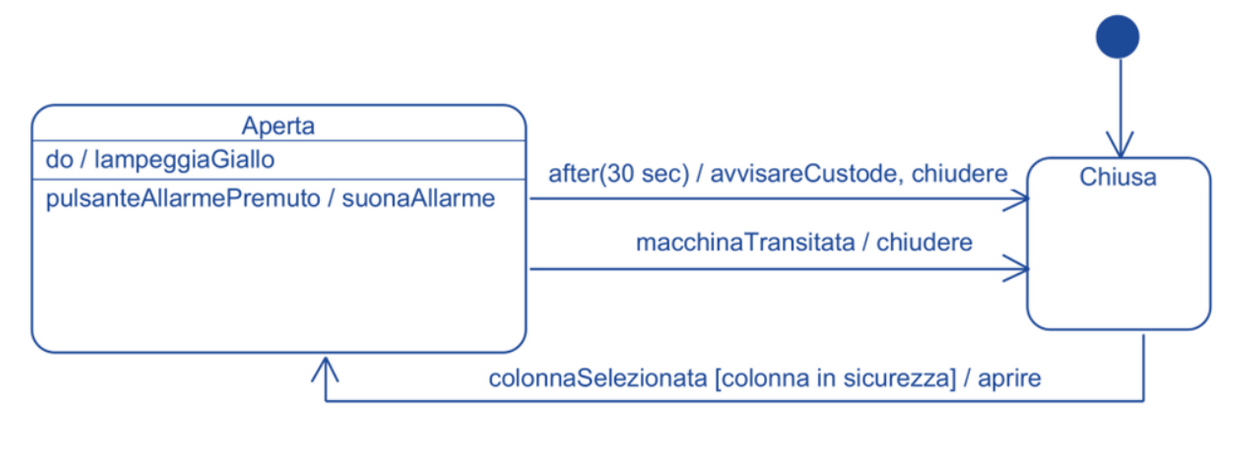
\includegraphics[scale=0.3]{dmodellohousecars.png}
		\captionof{figure}{Modello dinamico}
	\end{center}
\end{example}

\subsection{Requisiti}
Un requisito è una proprietà che deve essere garantita dal sistema per soddisfare una necessità dell'utente.
\begin{definition}[IEEE definition]
	Un requisito è:
	\begin{itemize}
		\item Una condizione (o capacità) necessaria a un utente per risolvere un problema o raggiungere un obiettivo
		\item Una condizione (capacità) che deve essere soddisfatta/posseduta da un sistema per soddisfare un contratto, uno standard, una specifica, o altri documenti formali
	\end{itemize}
\end{definition}
\noindent I requisiti possono essere di due tipi (che devono rimanere separati):
\begin{itemize}
	\item \textbf{Funzionali}: descrivono le \textbf{funzionalità} che il sistema deve realizzare in termini di \textit{azioni}, \textit{risposte agli input} e \textit{comportamenti in casi particolari}.
	\item \textbf{Non funzionali}: descrivono le \textbf{proprietà} del SW:
	\begin{itemize}
		\item \textbf{qualità}, e.g. efficienza, affidabilità, sicurezza
		\item \textbf{processo}, e.g. standard di processo, linguaggi usati, metodo di sviluppo
		\item \textbf{esterne}, e.g. interoperabilità e vincoli legislativi
		\item \textbf{fisici}, e.g. hardware, rete
	\end{itemize}
\end{itemize}
\begin{observation}
	Un requisito deve essere \textbf{ben posto}, idealmente nella forma \textbf{assertiva}
	\begin{equation*}
		\text{Il } <\text{sistema}>\text{ deve }<\text{funzionalità/proprietà}>
	\end{equation*}
\end{observation}

\begin{definition}[Documento dei requisiti]
	È un documento che specifica \textbf{cosa} deve fare il sistema e con quali \textbf{vincoli}. È un contratto tra lo sviluppatore e l'utente che in genere specifica anche la scadenza.
\end{definition}

\subsubsection{Acquisizione}
L'acquisizione può avvenire in diversi modi:
\begin{itemize}
	\item \textbf{Interviste}
	\begin{itemize}
		\item \textit{Strutturate}
		\item \textit{Non strutturate}
	\end{itemize}
	\item \textbf{Questionari} a risposta multipla
	\item Costruzione di \textbf{prototipi} (anche su carta)
	\item \textbf{Osservazione} di futuri utenti al lavoro: i \textbf{casi d'uso} devono includere la sequenza di eventi corretta ed eventuali comportamenti inattesi
	\item \textbf{User stories}: utilizzato nei processi \textit{Agile}, i requisiti sono descritti con un template predefinito
	\begin{equation*}
		\text{As a} <\text{user role}>\text{ I want }<\text{goal}>\text{ so that }<\text{benefit}>
	\end{equation*}
	che viene messo su un foglio in formato $A6$ (facile, visibile e rende possibile appenderli e collegarli). Questa tecnica però non è \textbf{scalabile}, è \textbf{vaga} e \textbf{informale} e spesso non include dettagli sui requisiti \textbf{non funzionali}.
	\item \textbf{Studio} di documenti
\end{itemize}

\subsubsection{Elaborazione}
Durante questa fase i requisiti vengono \textbf{espansi} e \textbf{raffinati} e viene scritta la prima bozza del documento. Questo deve essere strutturato in:
\begin{enumerate}
	\item \textbf{Introduzione}: perché il sistema è desiderabile e come si inquadra negli obiettivi più generali del cliente
	\item \textbf{Glossario}
	\item \textbf{Requisiti funzionali}
	\item \textbf{Requisiti non funzionali}
	\item \textbf{Architettura}: strutturazione in sottoinsiemi
	\item Specifica dei requisiti del software: specifica dettagliata dei requisiti \textbf{funzionali}
	\item \textbf{Modelli astratti} del sistema, formali o semi-formali
	\item \textbf{Evoluzione}: modifiche previste
	\item \textbf{Appendici}: individuazione ed eventuale descrizione della piattaforma hardware, requisiti di database, manuale utente, piani di test
	\item \textbf{Indici}
\end{enumerate}

\subsubsection{Convalida}
In questa fase si controlla il documento dei requisiti per evitare i seguenti errori:
\begin{itemize}
	\item \textbf{Omissioni} o incompletezza: mancata presenza di un requisito
	\item \textbf{Inconsistenza}: contraddizione tra i requisiti o tra un requisito e l'ambiente di lavoro
	\item \textbf{Ambiguità}: significati multipli. In particolare si deve prestare attenzione a:
	\begin{itemize}
		\item \textbf{Quantificatori}: e.g. tutti, sempre, ogni, niente, ogni, qualsiasi
		\item \textbf{Disgiunzioni}: e.g. AND, OR, XOR
		\item \textbf{Coordinazione}: e.g. \textit{Viaggerò in treno o in traghetto e in macchina}
		\item \textbf{Referenziale e anafore}: in base ai pronomi e a come vengono utilizzati
		\item \textbf{Vaghezze}: quando vengono usati \textit{aggettivi qualificativi} o \textit{avverbi non misurabili} (e.g. \textit{appropriato})
		\item \textbf{Verbi deboli} e \textbf{forme passive}: e.g. \textit{potere} oppure forme passive senza complemento di agente
	\end{itemize}
	\item \textbf{Sinonimi ed omonimi}
	\item Non devono esserci \textbf{dettagli tecnici}
	\item \textbf{Ridondanze} in una stessa sezione
\end{itemize}

\begin{note}
	Non usare doppie negazioni.
\end{note}

\noindent Per validare un documento già strutturato esistono varie tecniche.
\paragraph{Walkthrough}: lettura sequenziale dei documenti.
\paragraph{Lemmario}: si utilizzano i termini del glossario con puntatori ai requisiti che li nominano, aiutando a trovare \textit{inconsistenze}, \textit{omonimi}, \textit{sinonimi} e \textit{ridondanze}.
\paragraph{Natural Language Processing}: software che fanno un'analisi del documento alla ricerca di errori. Alcuni esempi sono: QuARs, TIGER-PRO e RQA
\paragraph{Prototipi}: presentazione di prototipi al committente

\begin{note}
	Eventuali errori di quelli sopra descritti devono sempre essere discussi con il cliente.
\end{note}

\subsubsection{Negoziazione}
In questa fase si assegnano delle \textbf{priorità} ai requisiti basandosi sulle \textbf{esigenze} del committente e sui \textbf{costi} e \textbf{tempi} di produzione. Durante questa fase alcuni requisiti possono essere cancellati o  posticipati.

\paragraph{MoSCoW} Questa tecnica assegna una priorità ai requisiti dividendoli nelle seguenti classi:
\begin{itemize}
	\item \textbf{Must have}: obbligatori e irrinunciabili per il cliente
	\item \textbf{Should have}: non necessari ma utili
	\item \textbf{Could have}: opzionali ma relativamente utili
	\item \textbf{Want to have}: contrattabili per successive versioni
\end{itemize}

\subsubsection{Gestione}
Per gestire i requisiti è fondamentale assegnargli un \textbf{identificatore univoco} oltre che diversi attributi:
\begin{itemize}
	\item \textbf{Stato}: proposto, approvato, rifiutato o incorporato
	\item \textbf{Priorità}
	\item \textbf{Effort} espresso in giorni e personale
	\item \textbf{Rischio} da un punto di vista tecnico
	\item \textbf{Stabilità}
	\item \textbf{Versione} di destinazione
\end{itemize}
È importante che i requisiti siano \textbf{tracciabili} per poter risalire ai \textit{componenti del sistema}, al loro \textit{codice} e ai \textit{test}.

\begin{note}
	È importante allegare il documento dei requisiti al contratto o, nel caso in cui non sia ancora pronto, prevedere una rinegoziazione.
\end{note}